\begin{figure*} 
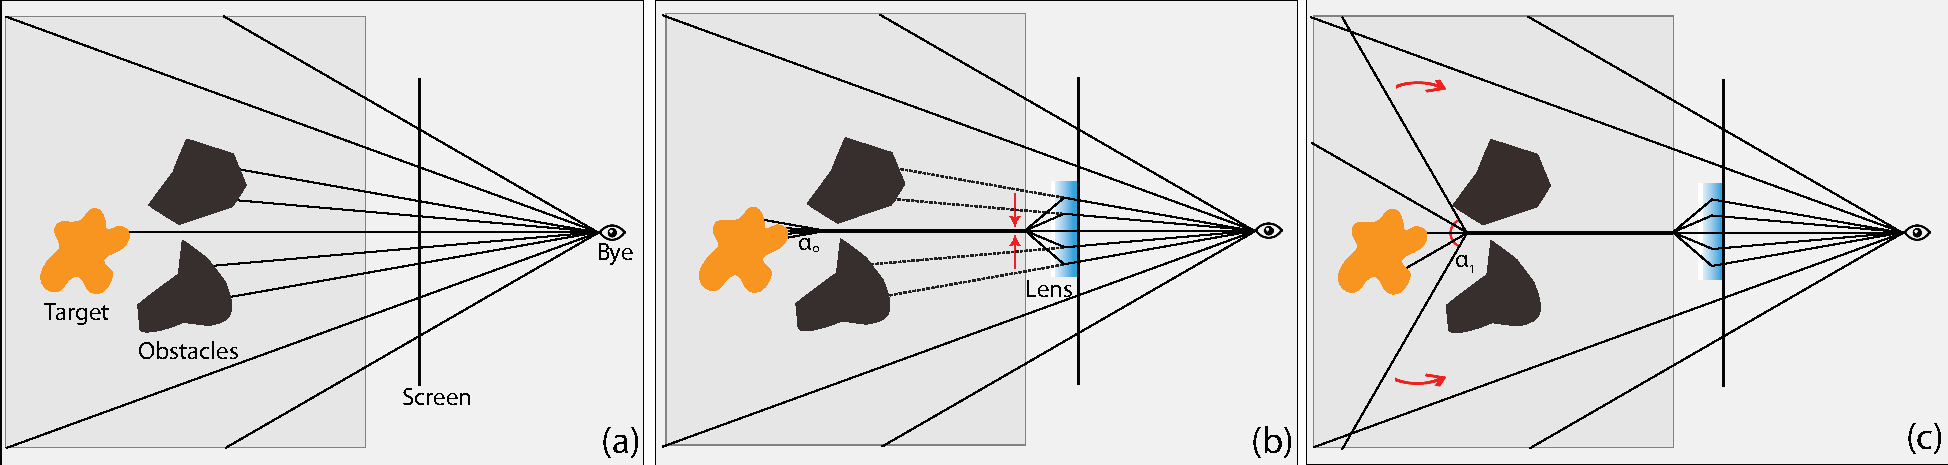
\includegraphics [width=\textwidth]{images/principle.pdf} 
\caption{The mechanism of the obstruction-free fish-eye lens. (a) The classic ray-casting where an interesting feature is partially hidden by other items in front of it. (b) The first main step: The lens makes converge the rays to avoid the obstacles. Once they are close to the target, the rays follow again their initial trajectory (with the initial angle) of view $\alpha_0$. Only a small part of the target is visible and magnified. (c) The target become visible by increasing the angle of view to $\alpha_1 \in \left[120,180\right]$.   }
\label{f:fisheye}
\end{figure*}


Direct volume rendering (DVR) is a pervasive visualization technique for displaying 3D scalar fields in many application fields such as engineering, material sciences, and medical imaging sciences. Recent DVR methods are able to display large such scalar fields at interactive rates and allow exploration of structures of interest. However widely adopted, and able to accommodate large volumes of data, DVR inherently suffers from the problem of \emph{occlusion}: Structures of interest located deep in the volume can be hard to spot and/or explore.

To aid with this, various mechanisms have been designed including transfer functions, segmentation, selection, and clipping. However, all such mechanisms have limitations.  \emph{Global} mechanisms, such as transfer function editing, can remove both occluders and objects of interest when these have similar densities. Moreover, in certain applications, carefully designed transfer functions exist and should be used without (significant) modifications to facilitate understanding and user training\,\cite{xxx}. \emph{Local} mechanisms such as segmentation, selection, or clipping are more effective in manipulating data confined to a given spatial region. However, many such mechanisms assume that one can easily and accurately select objects of interest to remove them (occluders) or keep them (occluded). This is hard to do when \emph{e.g.} one does not have direct access to the occluded objects, or when significant 3D interaction is required to select the occluder(s).


Many studies propose different tools and interaction techniques to by-pass occlusion issues in 3D environments such as lenses, deformations ~\cite{595268}, augmented reality, etc. Lenses, which are flexible lightweight tools that enable local and temporary modifications of the visualization, are suitable to deal with occlusion while keeping information about the global context. This is a good local solution for occlusion problems and an interesting way to keep the user aware of the global meaning of the dataset. Thus, while most lenses in volume rendering are used to magnify a volume subset~\cite{CGF:CGF12871}, we propose a focus+context (F+C) lens that combines a distortion technique which pushes aside the occluding objects, and a  fish-eye field of view in order to provide a better perspective on partially occluded items of interest in the volumes.  

A 

%ALEX: Removed below text, it's not really related to our contribution here
%Furthermore, performances are still a  challenge in volume rendering systems. In fact, depending on the size of the dataset and also the resolution of the resulting produced image: the rendering process can be very slow. Some optimization strategies such as empty space skipping~\cite{Liu:2009:AVR:2421899.2421919}, early ray termination~\cite{CGF:CGF12605}, multiple and adaptive resolutions allow to speed up the rendering process by increasing the frame rate. With the advent of CUDA as a higher-level GPU programming language, CUDA-based ray-casters were introduced~\cite{Kainz:2009:RCM:1661412.1618498}. 

So, in order to support our focus+context interactive lens, our volume visualization system relies on a CUDA-based ray-casting algorithm~\cite{Roettger:2003:SHV:769922.769948}.  This framework enables volumetric datasets visualization and offers a set of interactive tools including our lens for the purpose of easing the exploration and the manipulation of the data.

The structure of this paper is as follows. Section 2 presents related work in the areas of ray-casting, occlusion management, lenses and deformations. Section 3 describes the principle of our lens. Section 4 presents a method to convert vector datasets into a volume. Section 5 illustrates our lens technique with 3 scenarios. Section 6 discusses the presented technique. Finally, section 7 concludes the paper. 